%====================================================================%
%                  MORIOND.TEX                                       %
%====================================================================%

\documentclass{moriond}


\bibliographystyle{unsrt}    
% for BibTeX - sorted numerical labels by order of
% first citation.

% A useful Journal macro
\def\Journal#1#2#3#4{{#1} {\bf #2}, #3 (#4)}

% Some useful journal names
\def\NCA{\em Nuovo Cimento}
\def\NIM{\em Nucl. Instrum. Methods}
\def\NIMA{{\em Nucl. Instrum. Methods} A}
\def\NPB{{\em Nucl. Phys.} B}
\def\PLB{{\em Phys. Lett.}  B}
\def\PRL{\em Phys. Rev. Lett.}
\def\PRD{{\em Phys. Rev.} D}
\def\ZPC{{\em Z. Phys.} C}
\def\JINST{JINST}
\def\JHEP{JHEP}

% Some other macros used in the sample text
\def\st{\scriptstyle}
\def\sst{\scriptscriptstyle}
\def\mco{\multicolumn}
\def\epp{\epsilon^{\prime}}
\def\vep{\varepsilon}
\def\et{E_\textrm{T}^{\textrm{miss}}}
\def\ra{\rightarrow}
\def\ppg{\pi^+\pi^-\gamma}
\def\vp{{\bf p}}
\def\pt{{p_{\textrm{T}}}}
\def\ko{K^0}
\def\kb{\bar{K^0}}
\def\al{\alpha}
\def\ab{\bar{\alpha}}
\def\be{\begin{equation}}
\def\ee{\end{equation}}
\def\bea{\begin{eqnarray}}
\def\eea{\end{eqnarray}}
\def\CPbar{\hbox{{\rm CP}\hskip-1.80em{/}}}
%temp replacement due to no font
%%%%%%%%%%%%%%%%%%%%%%%%%%%%%%%%%%%%%%%%%%%%%%%%%%
%                                                %
%    BEGINNING OF TEXT                           %
%                                                %
%%%%%%%%%%%%%%%%%%%%%%%%%%%%%%%%%%%%%%%%%%%%%%%%%%

\newcommand{\Photo}{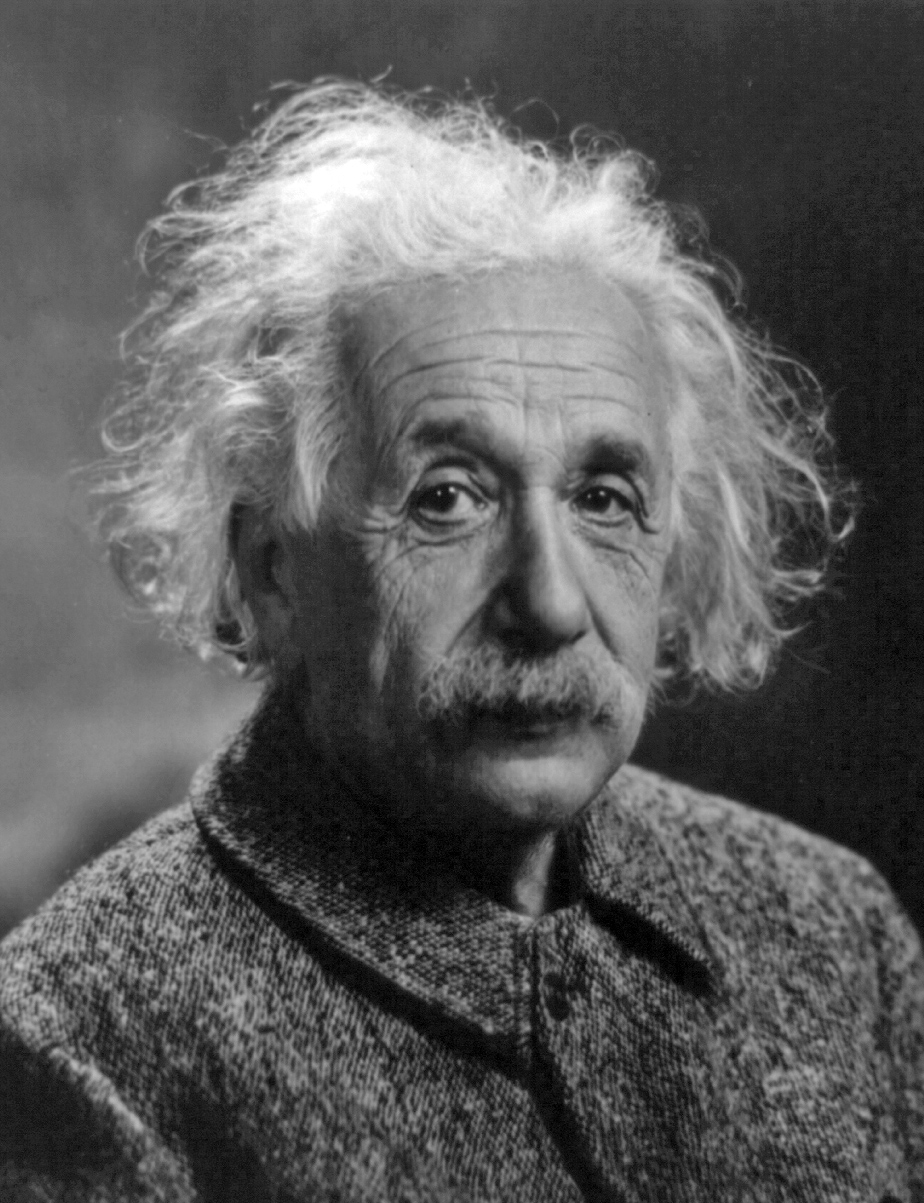
\includegraphics[height=35mm]{mypicture}}

\begin{document}
\vspace*{4cm}
\title{Searches for exotic Dark Matter at ATLAS and CMS}


\author{Bingxuan Liu, on behalf of the ATLAS and CMS Collaborations}

\address{Department of Physics, Simon Fraser University, Vancouver, Canada}

\maketitle\abstracts{The nature of dark matter is still a mystery. Many direct
and indirect search experiments are trying to solve this puzzle. The LHC offers
a unique opportunity at the high energy frontier, where dark matter particles
or related new particles may be produced and detected. Both the CMS and ATLAS
collaborations have carried out comprehensive dark matter search programs,
providing critical experiemntal results. In this article, recent exotic dark
matter searches in CMS and ATLAS are summarized and a brief outlook is given.}

\section{Introduction}

The nature of DM remains a mystery and there are many Beyond Standard Model
(BSM) theories proposed to offer an explanation. LHC~\cite{LHCRef} offers a
unique opportunity to search for Dark Matter (DM) and related new particles at
the high energy frontier.  ATLAS~\cite{ATLASRef} and CMS~\cite{CMSRef} are the
two general-purpose detectors at the LHC that are capable of searching for new
particles using a rich set of signatures. Both experiments have carried out
comprehensive dedicated DM search programs, primarily in the following
categories: 

\begin{itemize}
\item Mono-X Signature: DM candidates are produced in association with another detectable physics object (X). The non-interacting DM candidates give rise to a sizable missing transverse energy ($\et$). The detectable physics object can be a jet, photon, $Z$ boson and Higgs boson, or a Beyond Standard Model (BSM) particle that decays visibly.   
\item Resonance Signature: The mediator coupled to DM candidates is produced resonantly, decaying to SM particles to form a peak in the invariant mass spectrum. The SM pariticles can be a pair of jets, leptons or bosons. 
\item Associated Production with Heavy Flavor Quarks: DM candidates are produced in association with heavy flavor quarks, including a single top quark or a pair of top/bottom quarks. 
\item Supersymmetry (SUSY) Searches: DM candidates are produced in certain SUSY models which usually features a high jet multiplicity final state with a significant $\et$.  
\item SM Higgs Portal: DM candidates are decay products of the Higgs boson, where the Higgs boson is produced via SM processes. There is a sizable $\et$ recoiled against the visible physics objects which depends on the production mode of the Higgs boson such as the vecotr boson fusion (VBF). 
\end{itemize}    

The DM search program is expanding. The full LHC Run 2 data brings higher
precision to inclusive DM searches such as the mono-jet, mono-$Z$ and
mono-Higgs searches. More final states are being explored with aid from
innovative analysis techniques such as VBF + $\et$\ +
$\gamma$ and mono-s($\rightarrow VV$), motivated by theories such as dark
Higgs~\cite{DarkH} and dark photon~\cite{DarkPh}. In the meantime, the
theoretical framework has also advanced in the past decades, taking the
experiment results into account.  As a consequence, more models have thrived,
encouraging both CMS and ATLAS to provide more interpretations. In paricular,
the 2HDM + a model~\cite{2HDM} is widely considered in recent searches.
Figure~\ref{fig:diagrams} shows the diagrams of the models mentioned a bove.

\begin{figure} [htb]
\begin{minipage}{0.32\linewidth}
\centerline{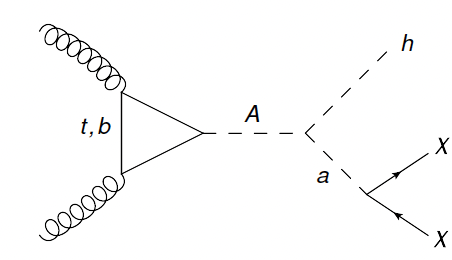
\includegraphics[width=0.9\linewidth]{2HDM_a}}
\end{minipage}
\begin{minipage}{0.32\linewidth}
\centerline{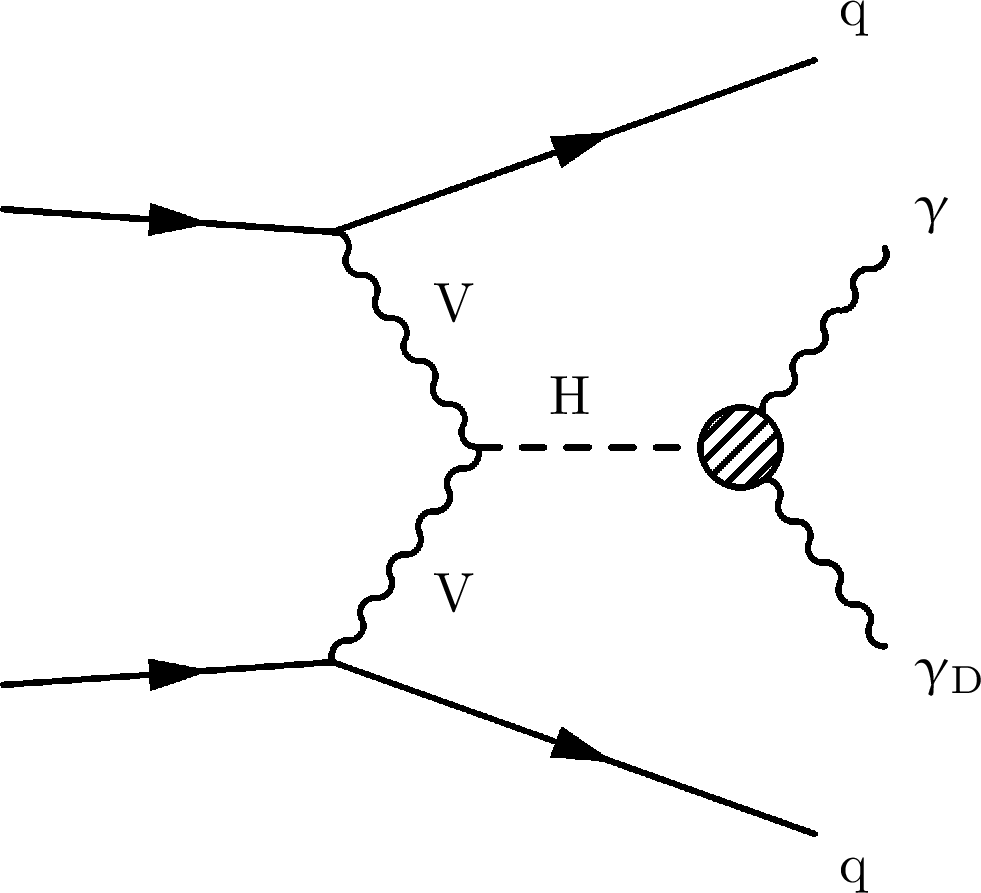
\includegraphics[width=0.9\linewidth]{HiggsDarkPhotonDiagram}}
\end{minipage}
\begin{minipage}{0.32\linewidth}
\centerline{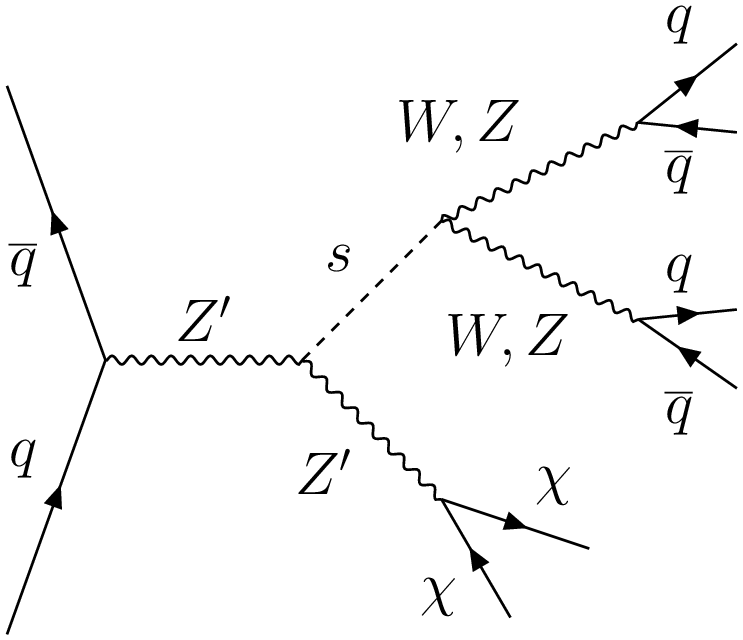
\includegraphics[width=0.9\linewidth]{MonoSVVDiagram}}
\end{minipage}
\caption[]{Diagrams of various models considered in recent DM searches. Left: A Higgs boson is produced in association with a pseudo-scalar decaying to DM candidates (2HDM + a); middle: a Higgs boson is produced in the VHF channel, decaying to a photon and a dark photon; right: a dark Higgs s is produced in association with a $Z/pime$, where the $Z/prime$ decays to DM candidates and the dark higgs s decays to two vectro bosons.}
\label{fig:diagrams}
\end{figure}

Recent results from both CMS and ATLAS will be summarized in the next section
followed by an outlook on the future DM seearch programs at the LHC.

\section{Dedicated search results}

\subsection{Mono-X searches}

Mono-jet search is the flagship analysis in the DM regime as its simple final
state covers a large range of parameter space, sensitive to many different
models. The recent ATLAS mono-jet search uses full Run 2 ATLAS data with an
integrated luminosity of 139 $\textrm{fb}^{-1}$, collected by a $\et$\ trigger.
The events are required to have at least one jet with transverse momentum
($\pt$) greater than 150 GeV and not have leptons or photons present. Signal
regions are divided by $\et$\ starting at 200 GeV. Various control regions are
constructed by including leptons in the selections to constrain the background
contributions via a simultaneous fit. 

Mono-$Z$ can be carried out in either the leptonic or hadronic final states.
The recent CMS mono-$Z$ search considers the leptonic final state where the $Z$
boson decays to either a pair of muons or electrons.  

\begin{figure} [htb]
\begin{minipage}{0.45\linewidth}
\centerline{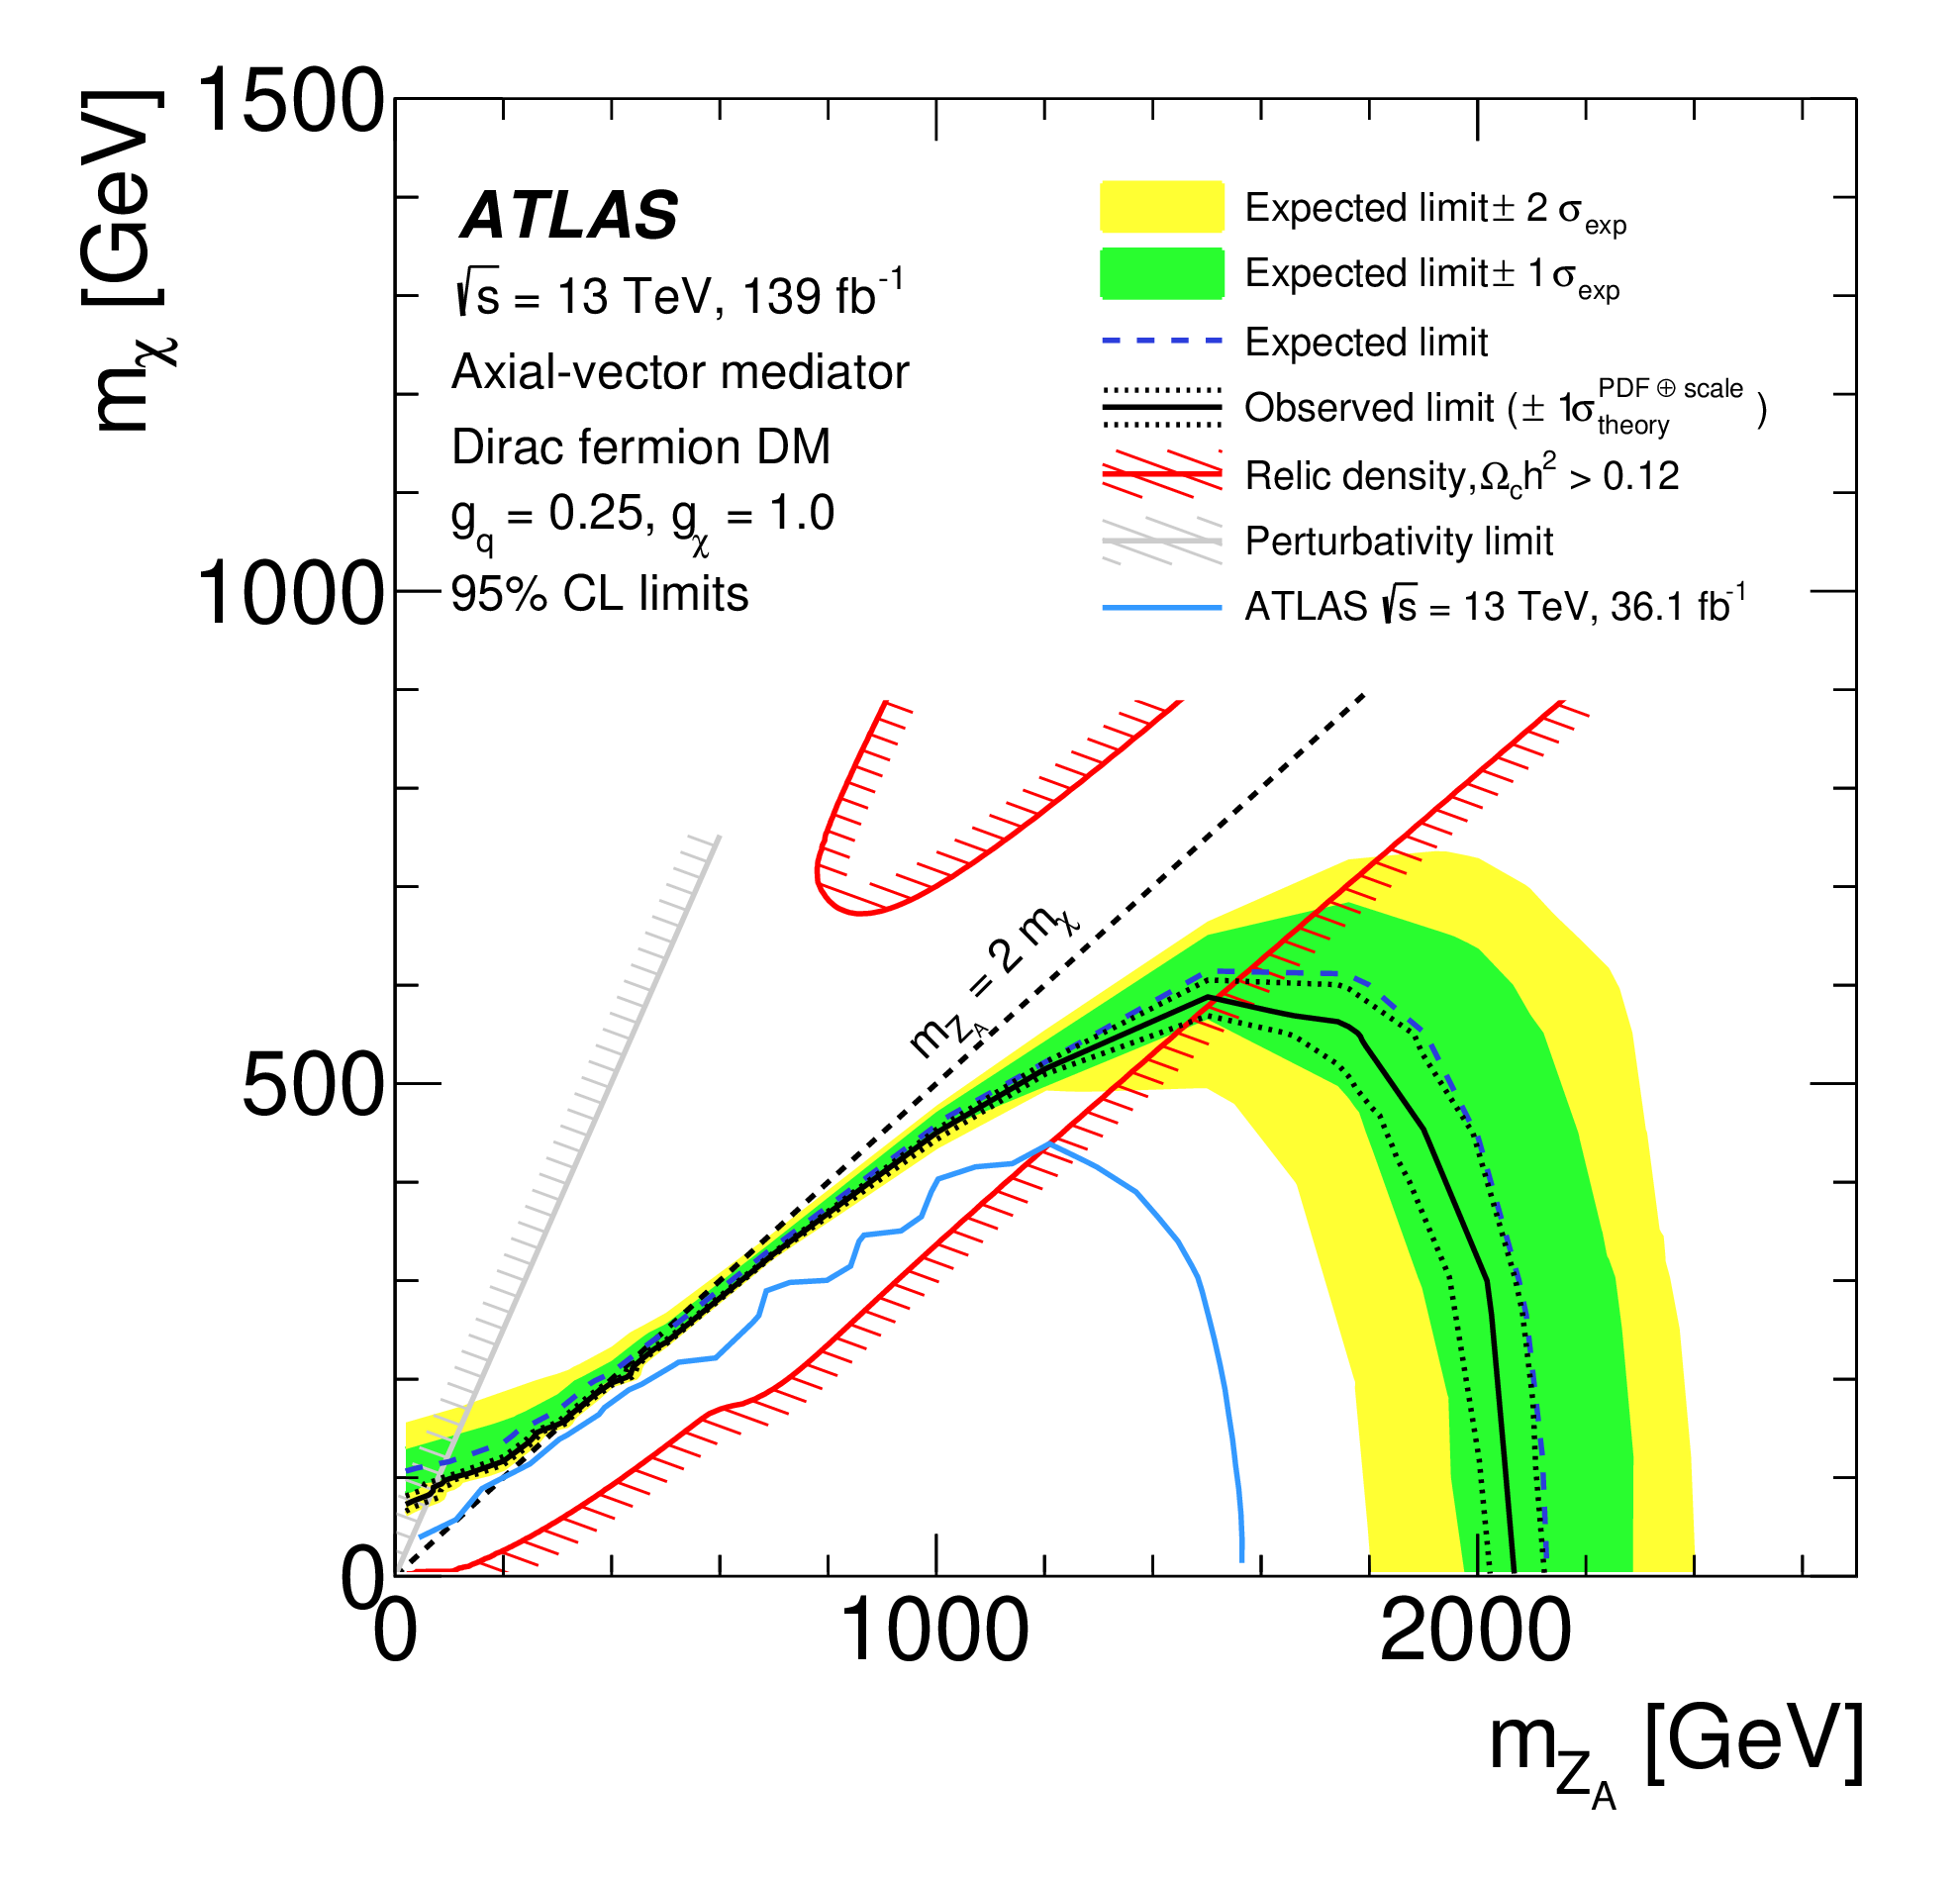
\includegraphics[width=0.9\linewidth]{monojet}}
\end{minipage}
\begin{minipage}{0.45\linewidth}
\centerline{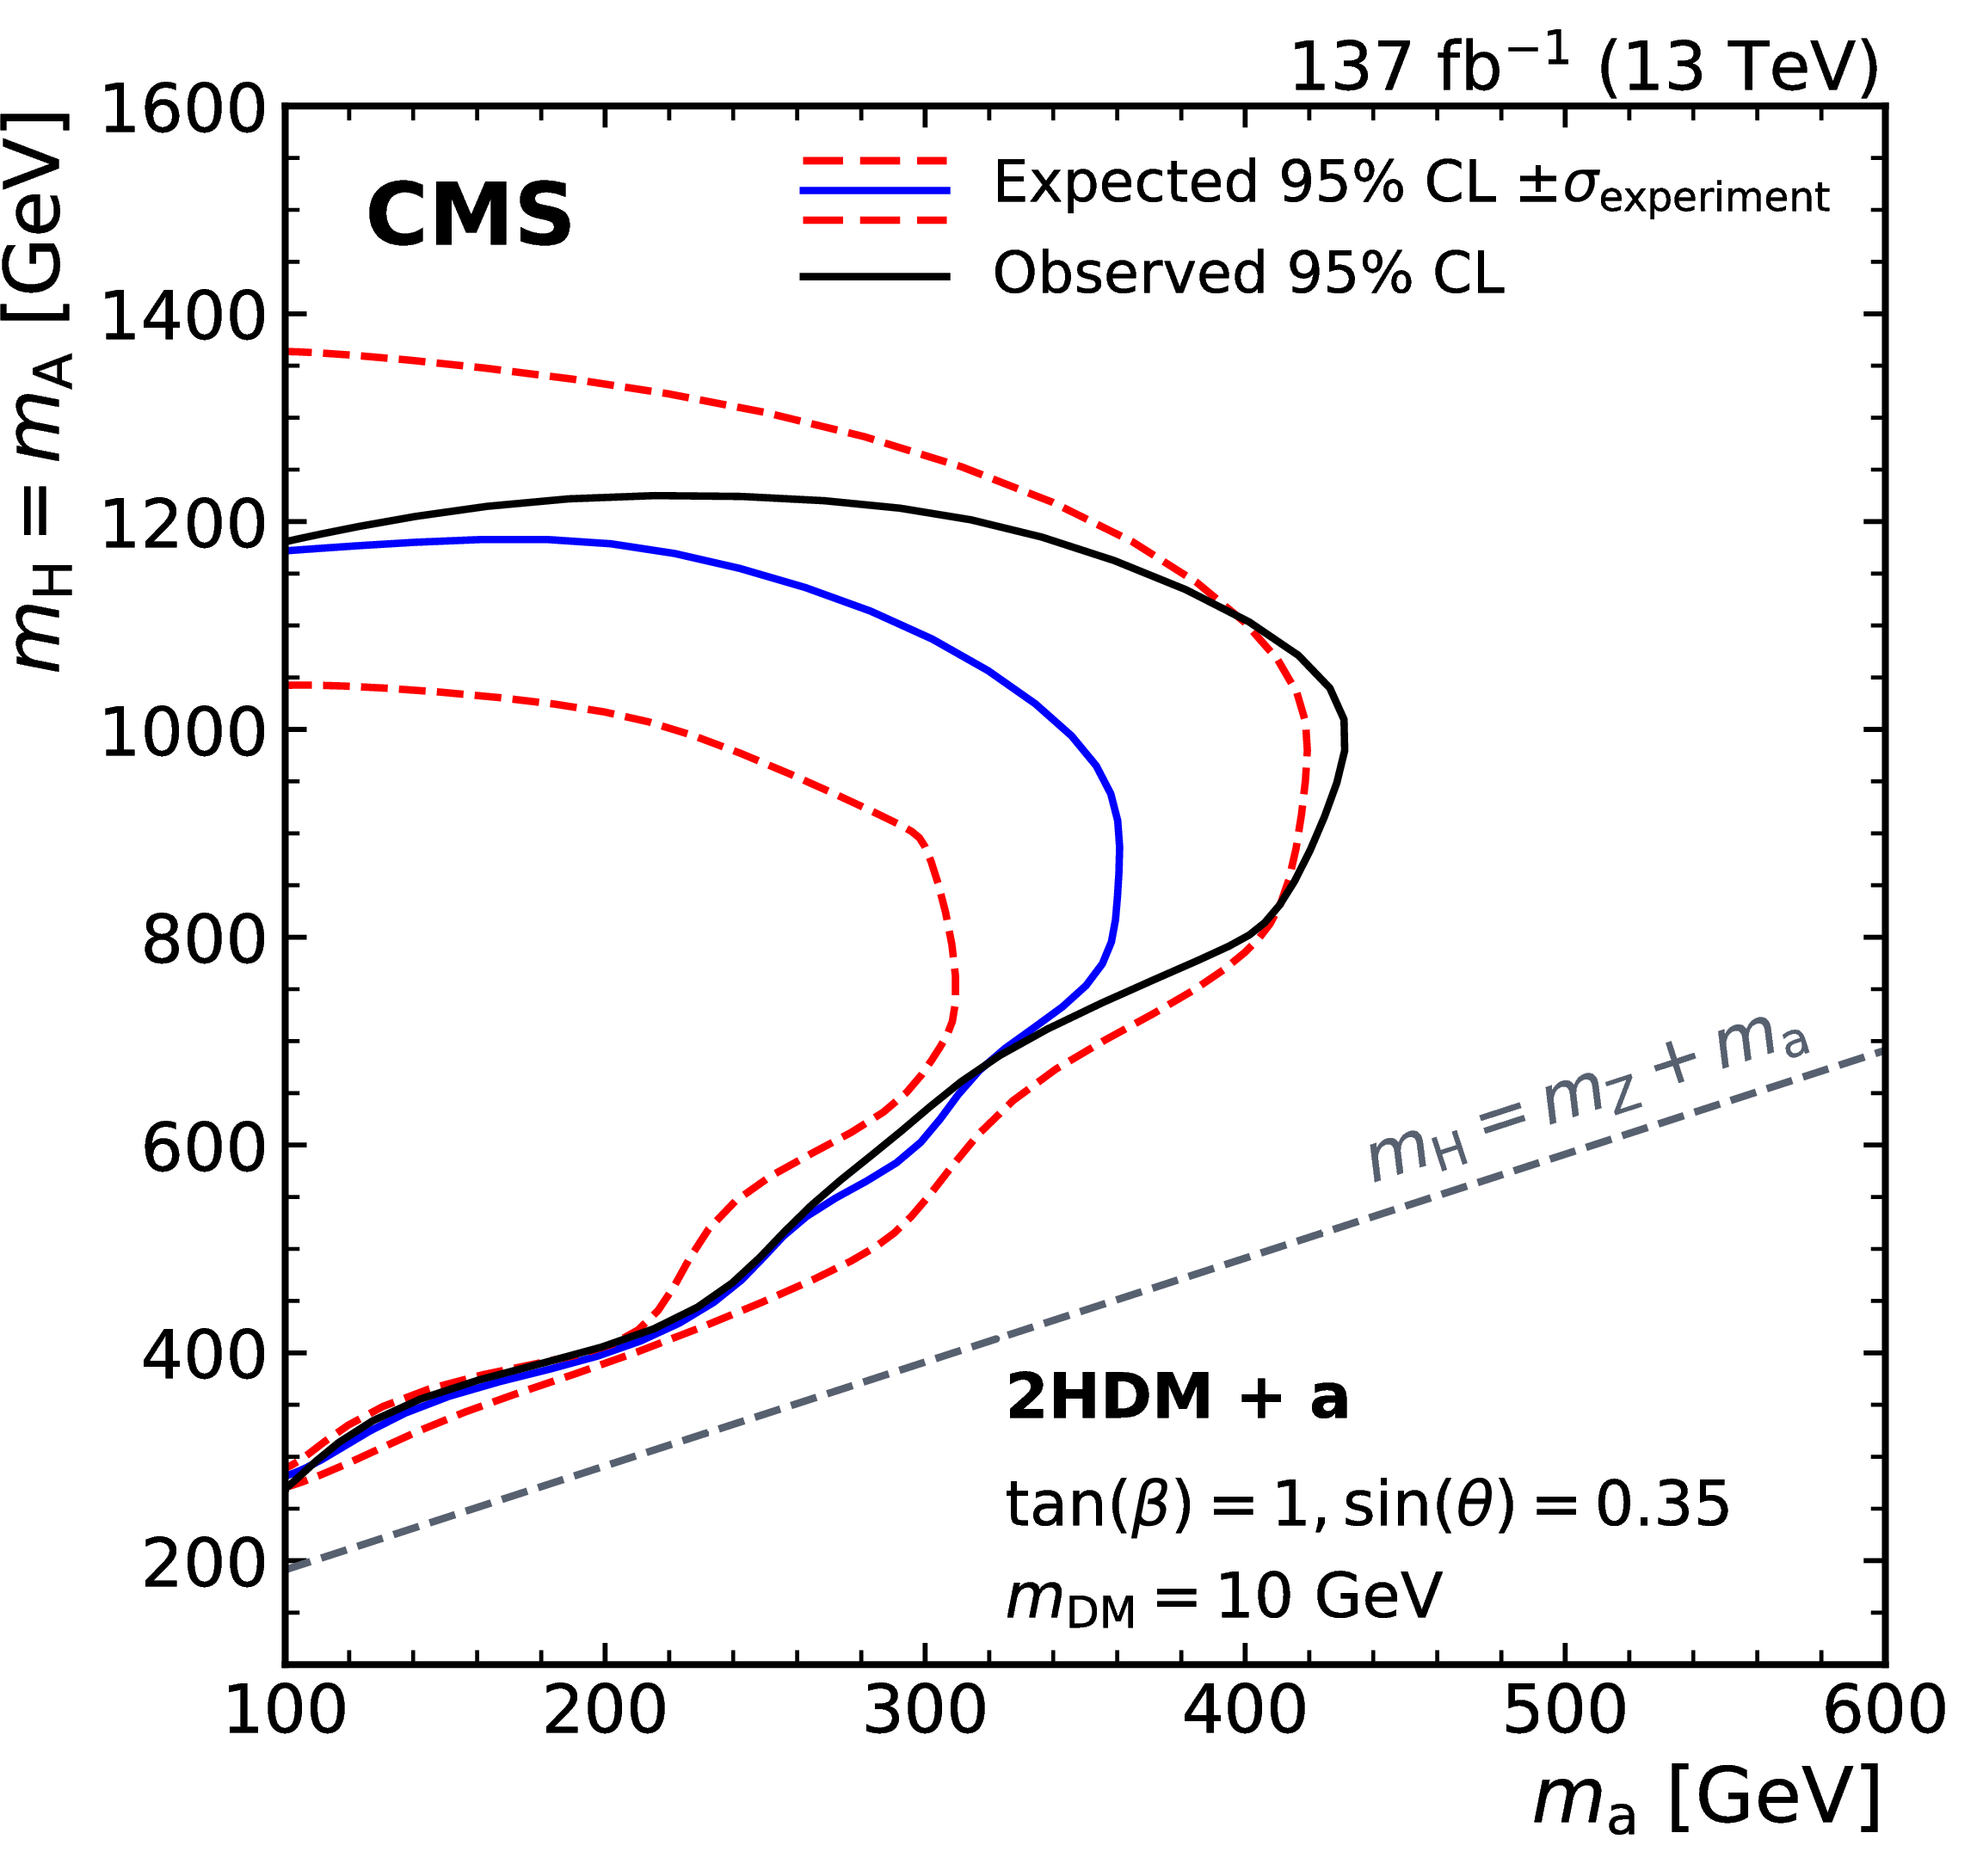
\includegraphics[width=0.9\linewidth]{monoz}}
\end{minipage}
\caption[]{}
\label{fig:mono_jet_z}
\end{figure}

\begin{figure} [htb]
\begin{minipage}{0.45\linewidth}
\centerline{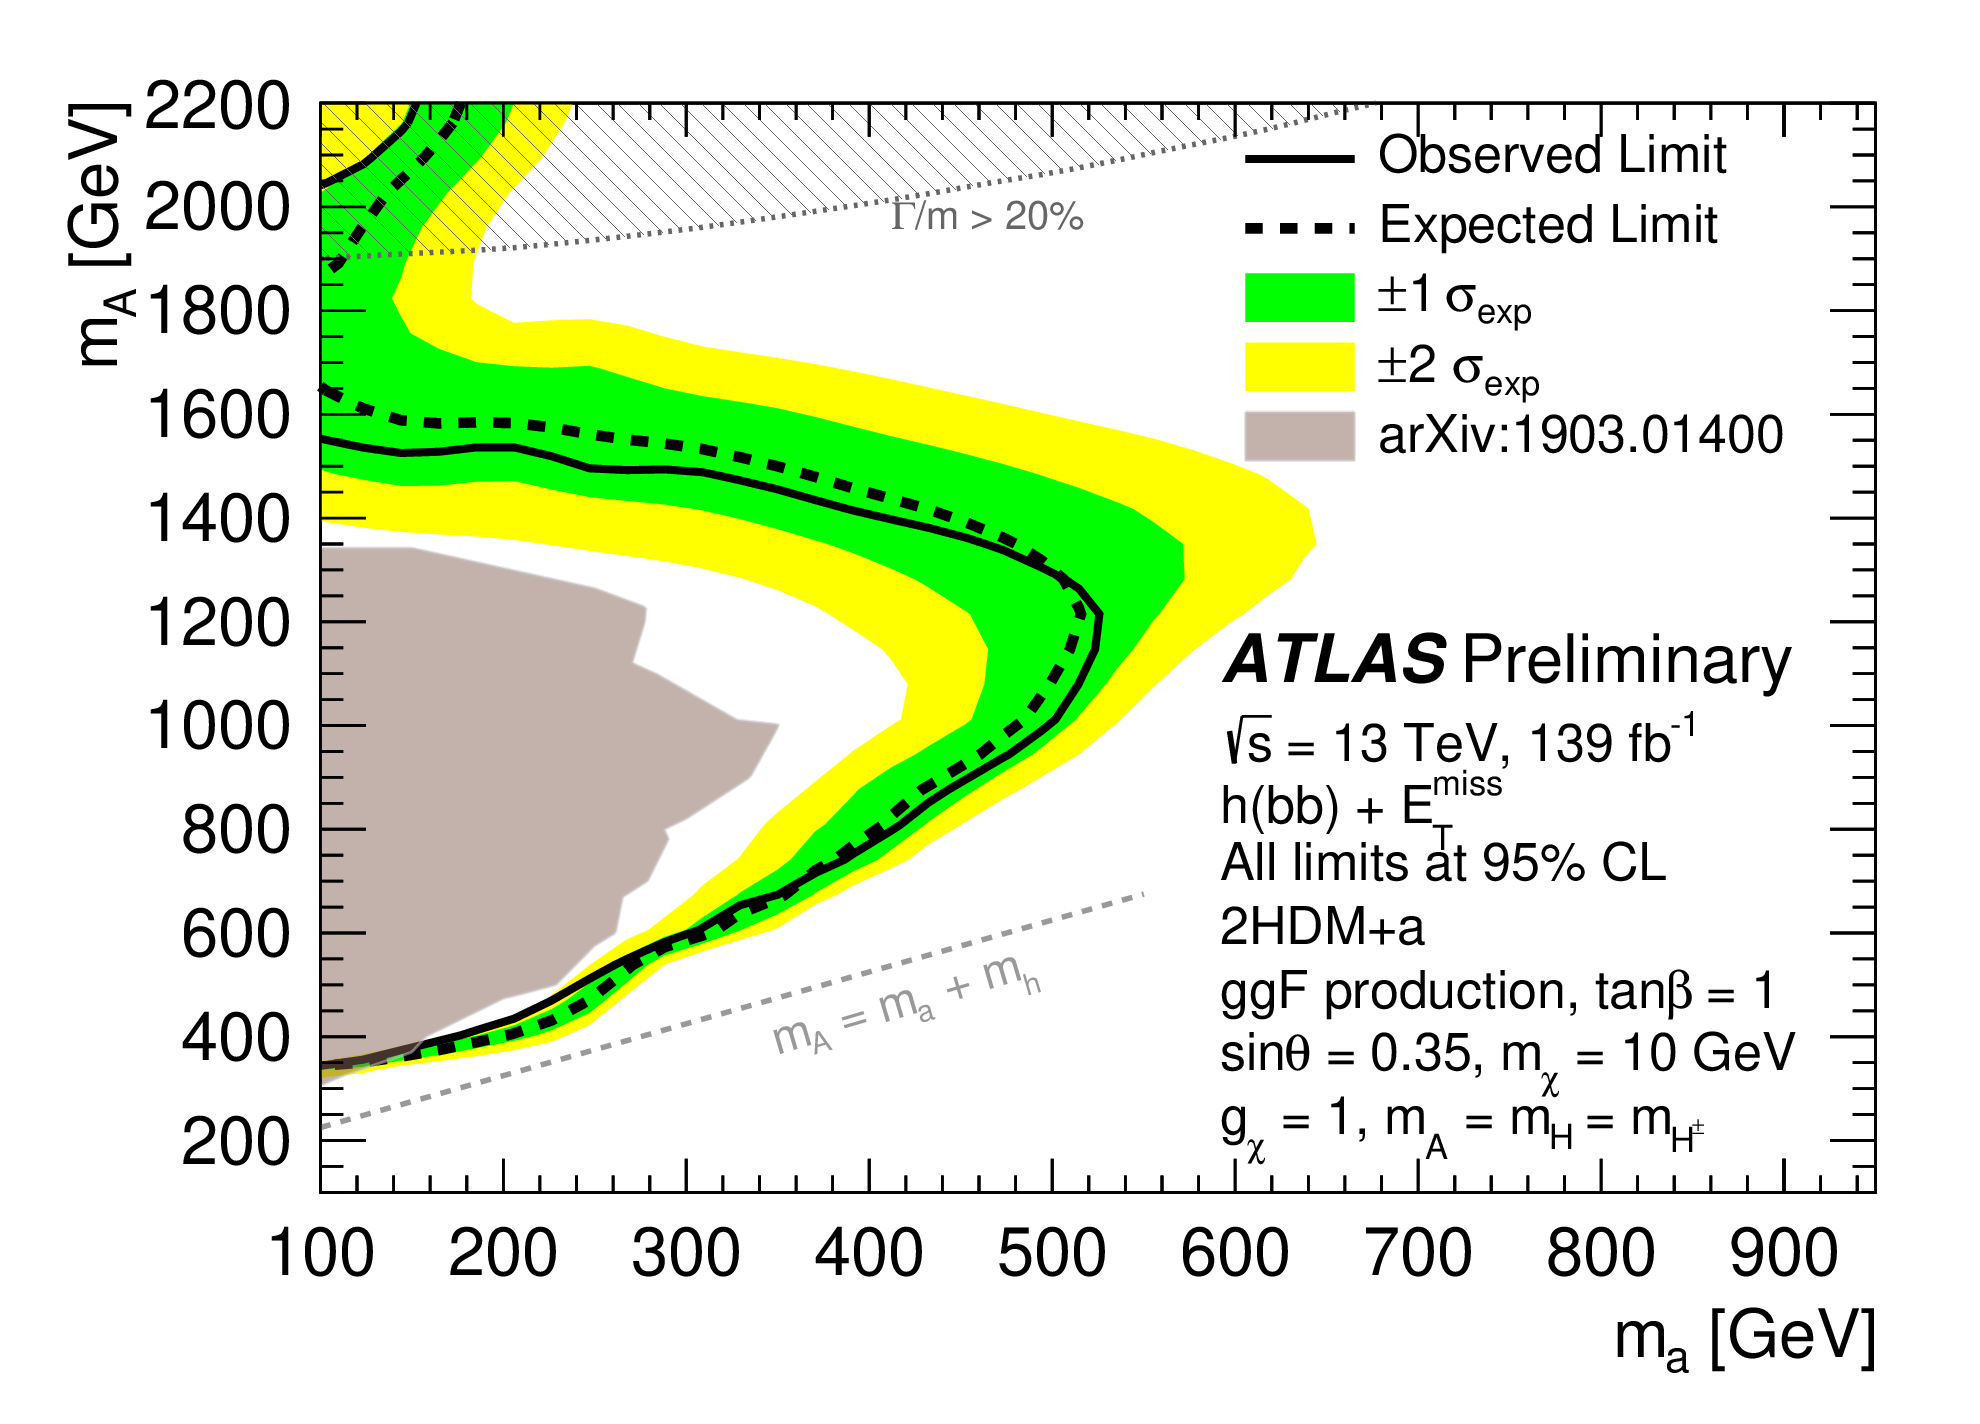
\includegraphics[width=0.9\linewidth]{monoh}}
\end{minipage}
\begin{minipage}{0.45\linewidth}
\centerline{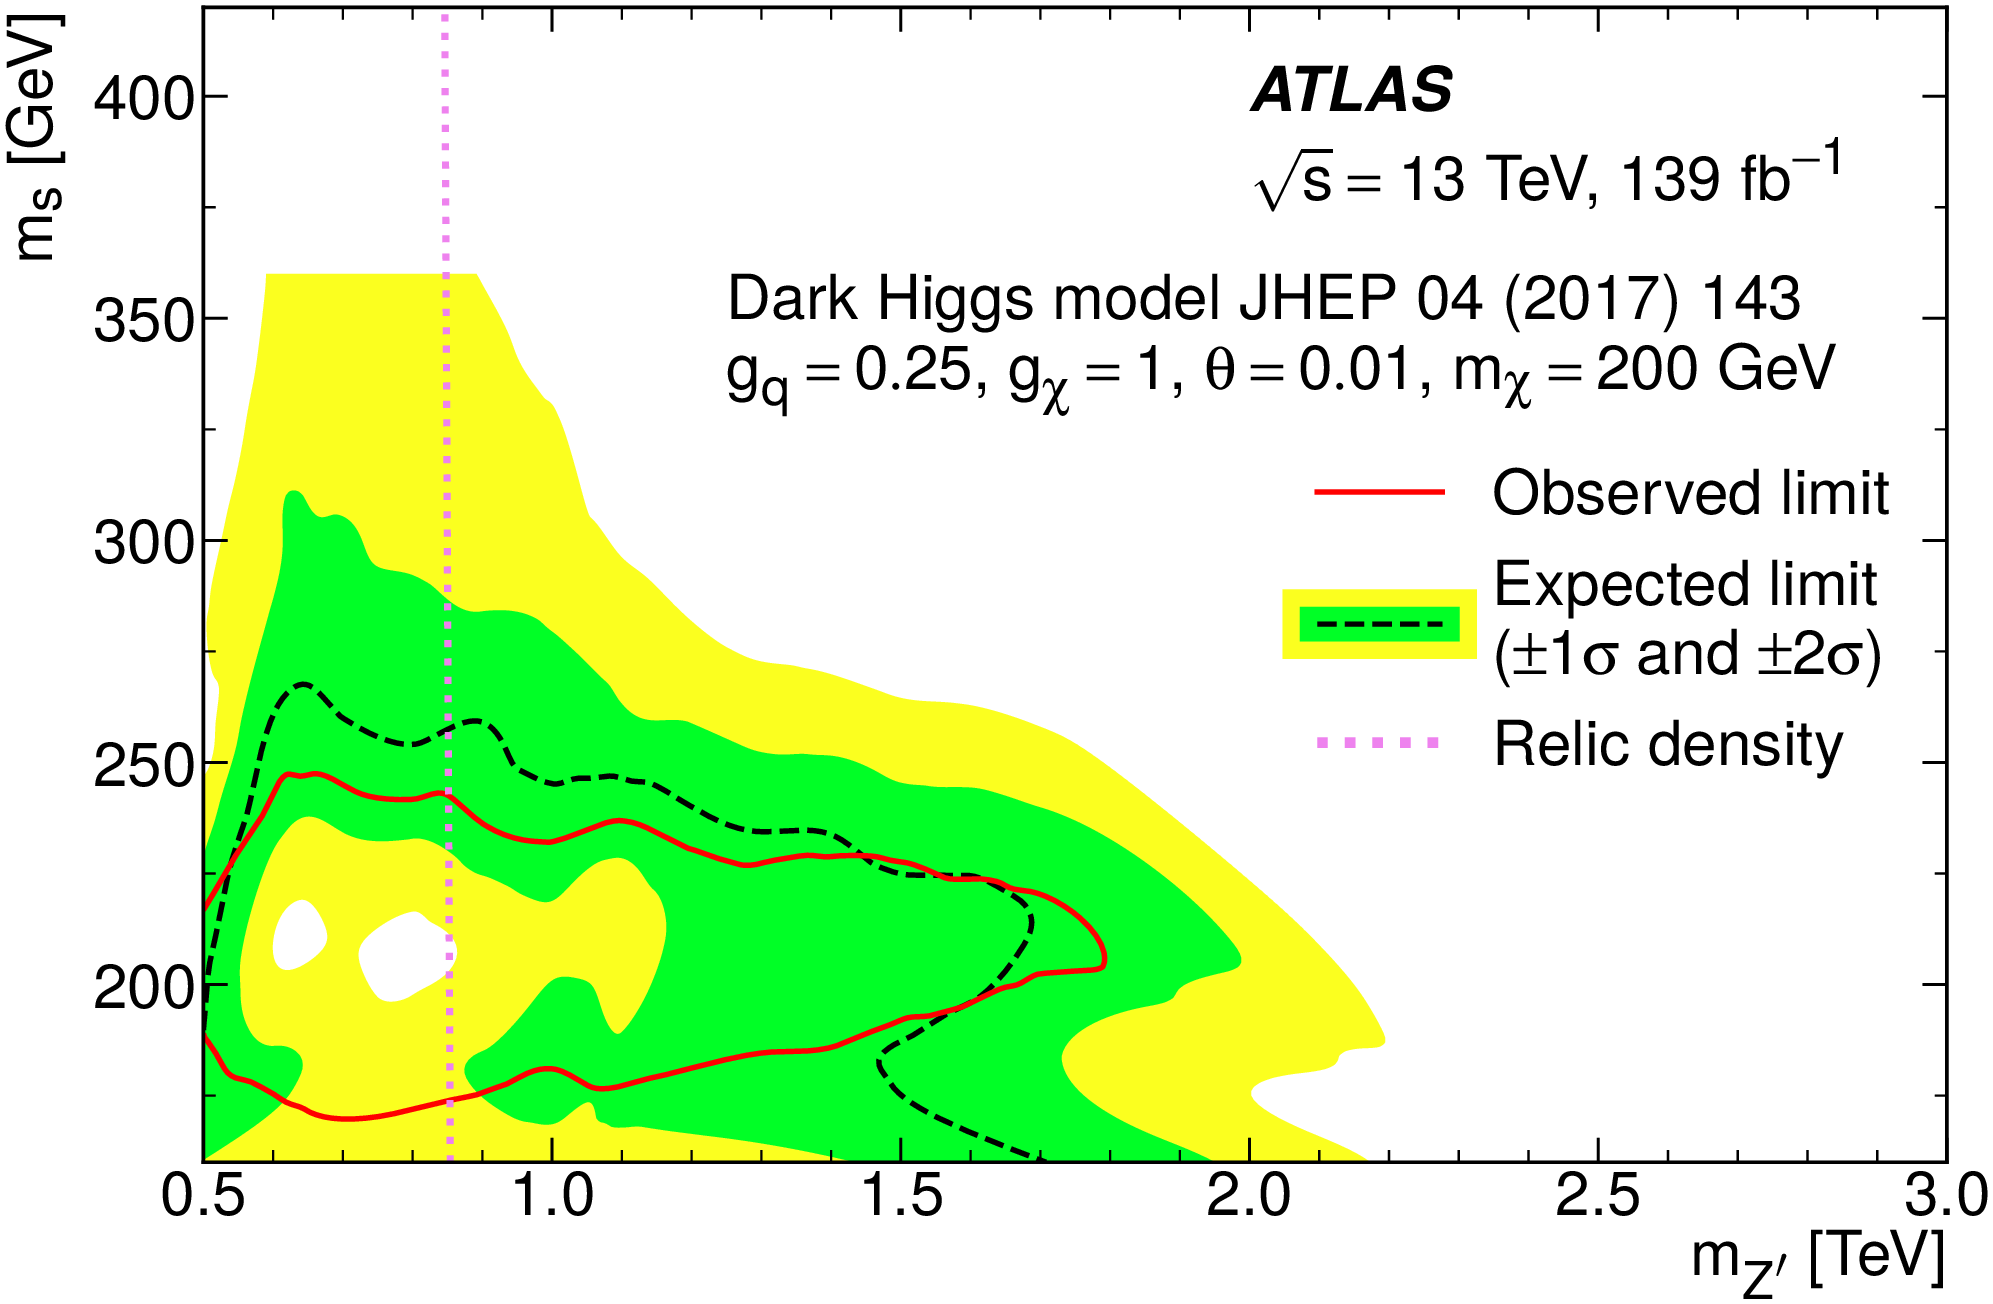
\includegraphics[width=0.9\linewidth]{monos}}
\end{minipage}
\caption[]{}
\label{fig:mono_h_s}
\end{figure}

\subsection{Dark photon search in the VBF channel}

\begin{figure} [htb]
\begin{minipage}{0.45\linewidth}
\centerline{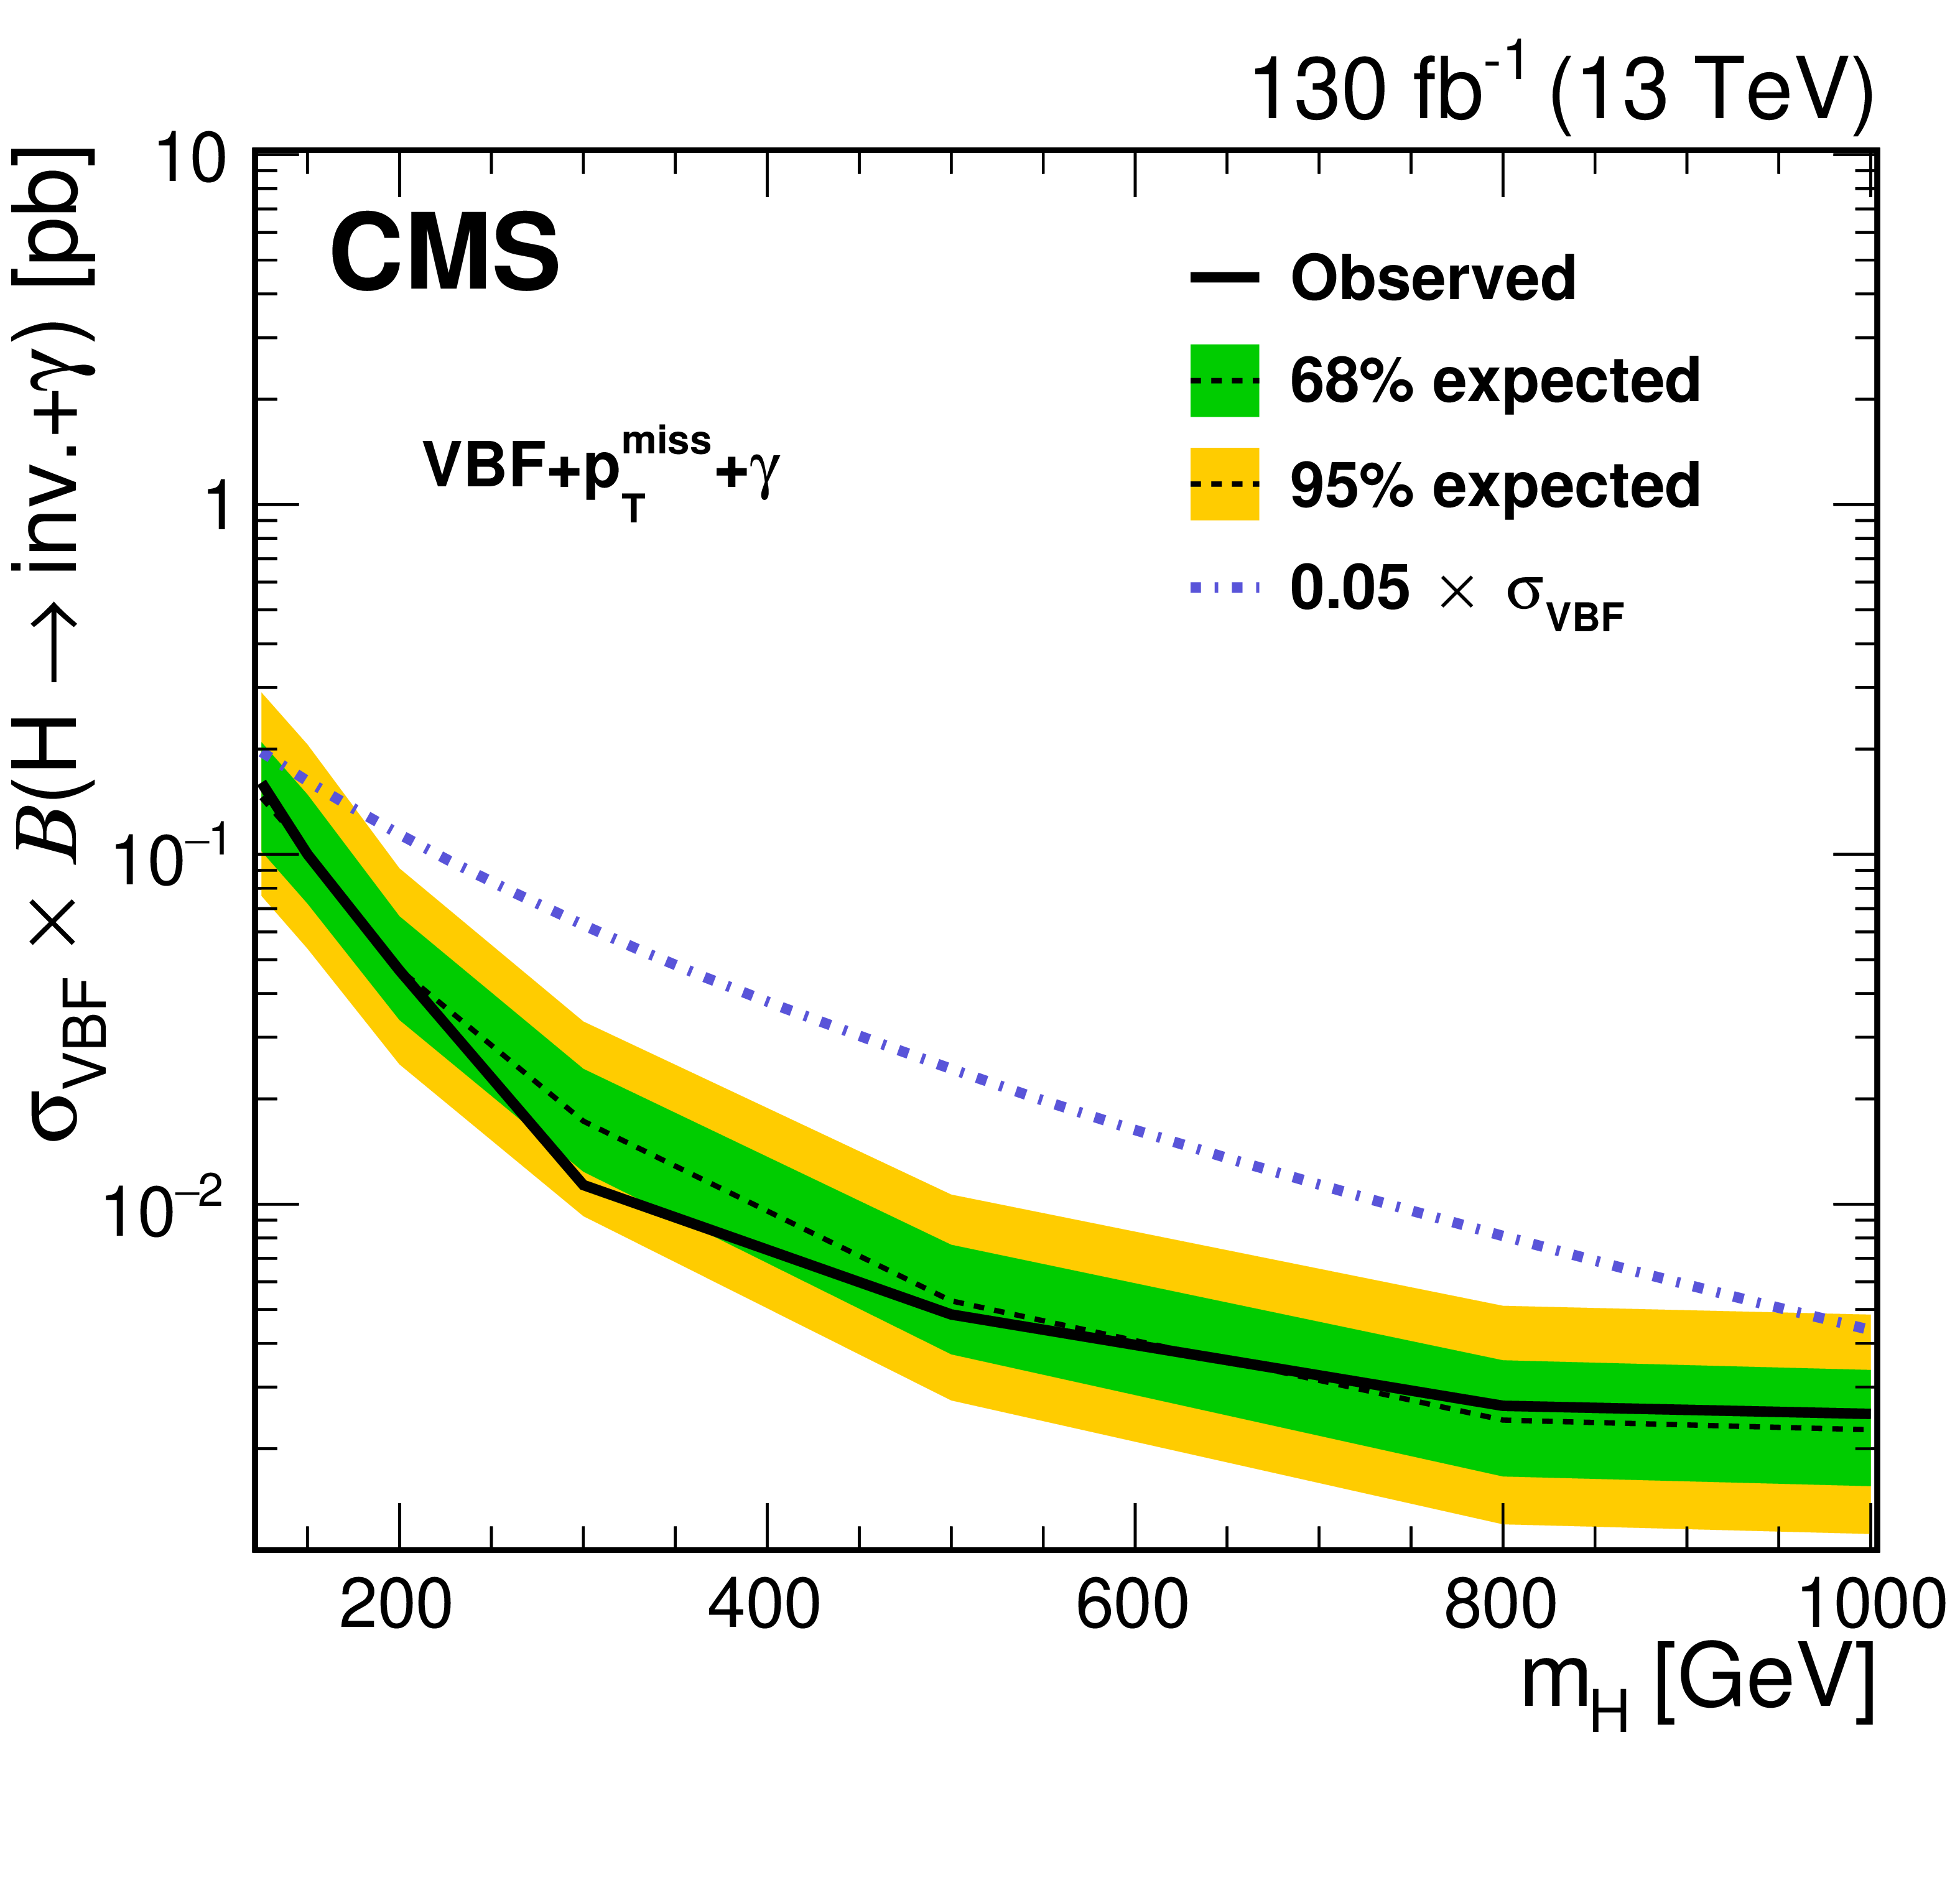
\includegraphics[width=0.9\linewidth]{cmsvbf}}
\end{minipage}
\begin{minipage}{0.45\linewidth}
\centerline{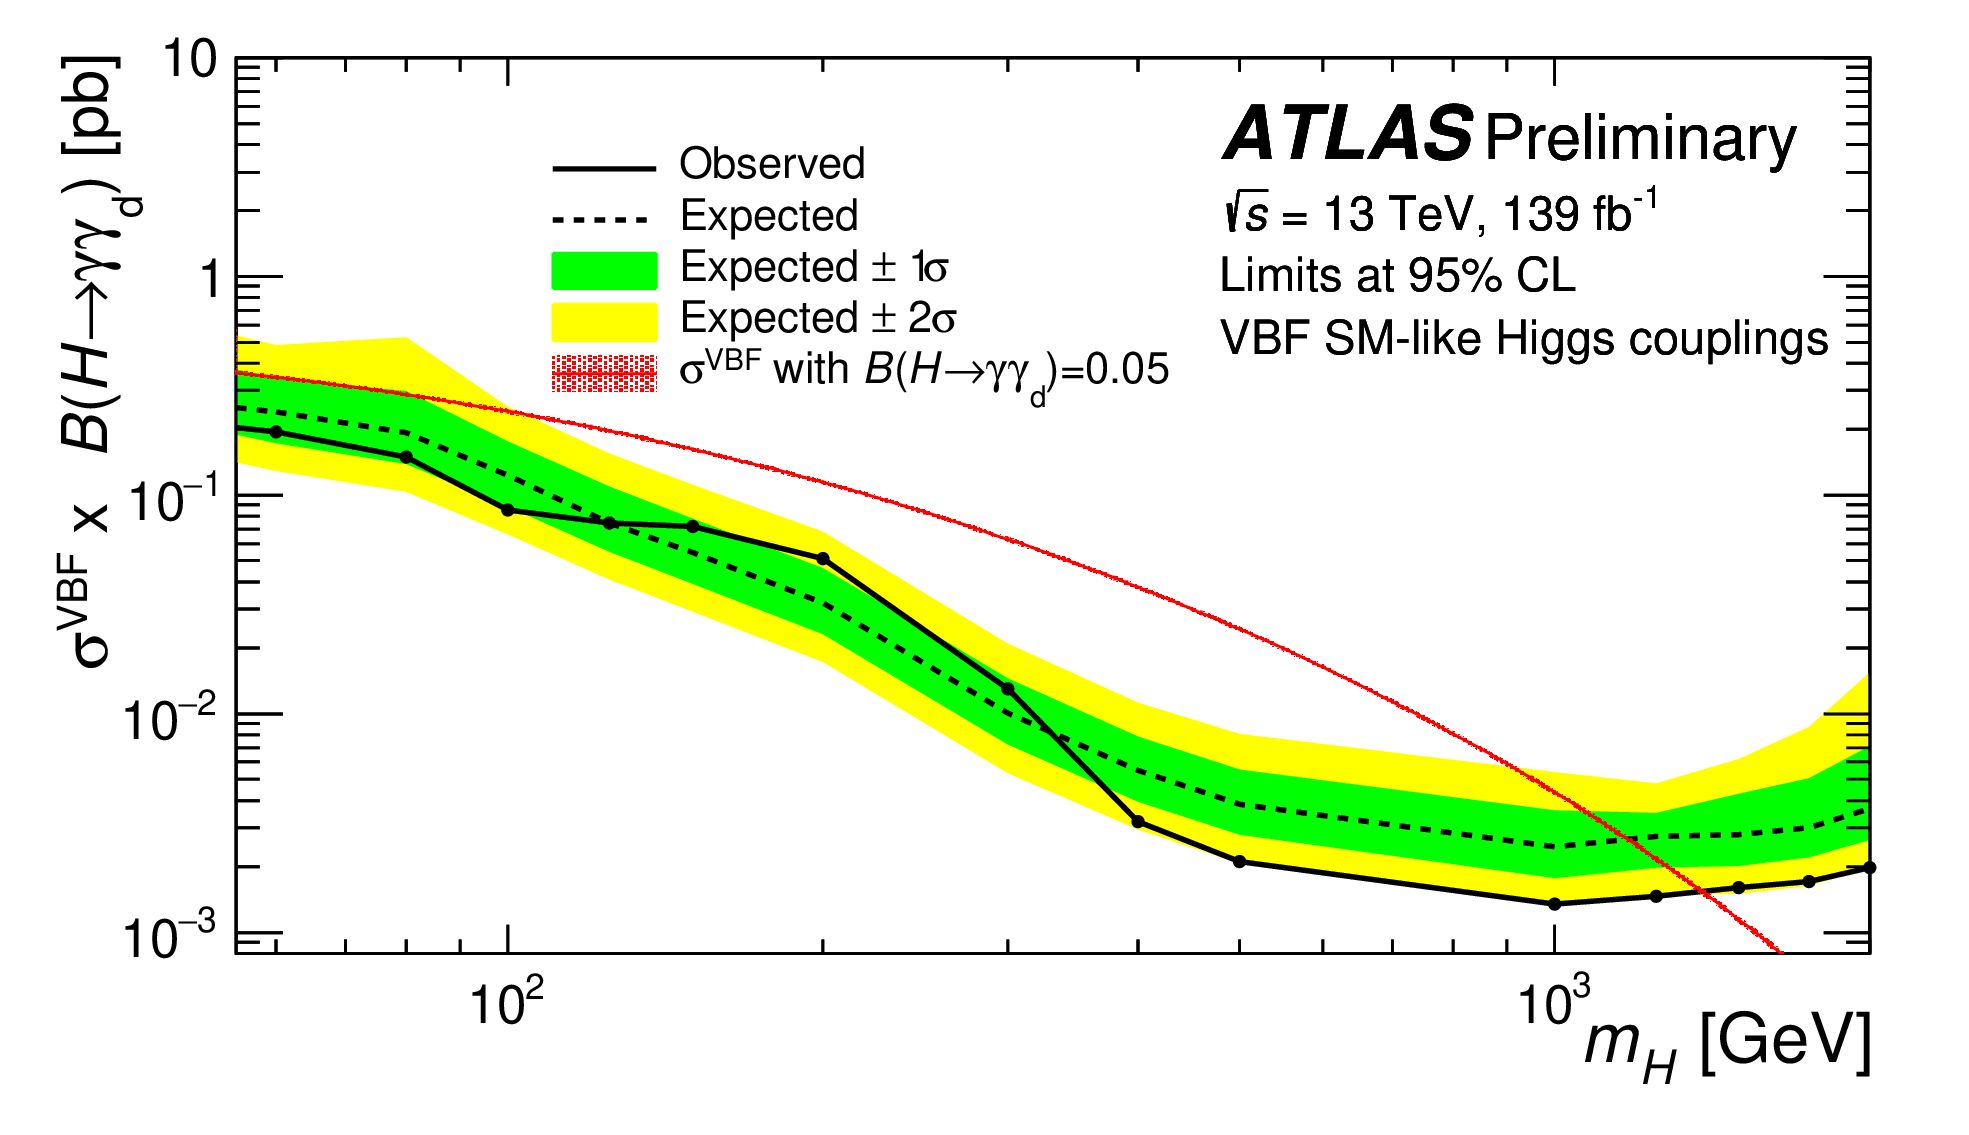
\includegraphics[width=0.9\linewidth]{atlasvbf}}
\end{minipage}
\caption[]{}
\label{fig:vbf}
\end{figure}

\subsection{DM interpretations in Susy searches}

\begin{figure} [htb]
\centerline{\includegraphics[width=0.5\linewidth]{DMBB}}
\caption[]{}
\label{fig:dmbb}
\end{figure}

\section{Conclusions}



\section*{References}

\begin{thebibliography}{99}
\bibitem{ja}C Jarlskog in {\em CP Violation}, ed. C Jarlskog
(World Scientific, Singapore, 1988).

\bibitem{LHCRef}L. Evans and P. Bryant (editors), \Journal{\JINST}{3}{S08001}{2008}.

\bibitem{CMSRef}CMS Collaboration, \Journal{\JINST}{3}{S08004}{2008}.

\bibitem{ATLASRef}ATLAS Collaboration, \Journal{\JINST}{3}{S08003}{2008}.

\bibitem{DarkH}Duerr, Michael and Grohsjean, Alexander and Kahlhoefer, Felix and Penning, Bjoern and Schmidt-Hoberg, Kai and Schwanenberger, Christian, \Journal{\JHEP}{04}{143}{2017}.

\bibitem{DarkPh}Biswas, Sanjoy and Gabrielli, Emidio and Heikinheimo, Matti and Mele, Barbara, \Journal{\PRD}{93}{093011}{2016}.

\bibitem{2HDM}Bauer, M., Haisch, U. and Kahlhoefer, F., \Journal{\JHEP}{05}{138}{2017}.

\end{thebibliography}

\end{document}

%%%%%%%%%%%%%%%%%%%%%%
% End of moriond.tex  %
%%%%%%%%%%%%%%%%%%%%%%


%%% Local Variables: 
%%% mode: latex
%%% TeX-master: t
%%% End: 

%%% Local Variables: 
%%% mode: latex
%%% TeX-master: t
%%% End: 

%%% Local Variables: 
%%% mode: latex
%%% TeX-master: t
%%% End: 
